\documentclass[10pt]{article}
\usepackage{iclr2026_conference}
\usepackage{amsmath,amssymb}
\usepackage{booktabs}
\usepackage{graphicx}
\usepackage{hyperref}
\usepackage{xcolor}

\title{Best-of-N Can Amplify Sparse-View Geometry Errors in 3D Scene World Models}

\begin{document}
\maketitle

\begin{abstract}
Learned 3D scene world models increasingly represent futures as neural fields,
Gaussian splats, point clouds, or occupancy volumes. A common inference pattern
is to sample multiple candidate futures and select the candidate with the best
proxy score. This paper studies a narrow failure mode of that pattern: when the
proxy observes only sparse views, Best-of-N selection can prefer candidates that
match the scored views while becoming less consistent in hidden 3D regions. We
build a deterministic synthetic voxel benchmark that isolates the mechanism.
Naive sparse-view Best-of-N improves proxy score from 0.791 at $N=1$ to 1.000
at $N=64$, but true 3D IoU falls from 0.520 to 0.340 and hidden-region error
rises from 0.442 to 0.929. A simple reranker using ensemble geometry consensus,
visual-hull volume plausibility, and surface-complexity penalties recovers much
of the hidden geometry, reaching 0.888 true IoU at $N=16$. The result is not a
claim that all neural scene models fail this way; it is a runnable diagnostic
for an under-tested interaction between sparse projective scoring and
multi-sample inference.
\end{abstract}

\section{Introduction}

Best-of-N inference is attractive for world models: sample several plausible
future scenes, score them with a task proxy, and execute or report the best. In
3D scene representations this proxy often comes from sparse observations:
rendered views, depth maps, partial point clouds, or task-relevant camera rays.
The proxy is cheaper and more available than full 3D ground truth, but it is not
injective. Many different 3D scenes can share the same silhouettes and visible
front surfaces.

This paper asks what happens when that ambiguity meets Best-of-N selection. The
answer in our controlled benchmark is uncomfortable: increasing $N$ can make the
selected candidate look better under the sparse proxy while making it worse as a
3D scene. The selector finds rare view impostors. These candidates are excellent
under the scored views and poor in hidden regions.

Our contribution is a mechanism-specific diagnostic rather than a new renderer:

\begin{itemize}
  \item a synthetic 3D scene-world benchmark with primitive occupancy scenes,
  stochastic candidate futures, sparse orthographic proxy views, and hidden
  geometry labels for evaluation;
  \item diagnostics for proxy score, true 3D IoU, hidden-region error,
  selected-candidate diversity, view-impostor rate, and the geometric
  exploitation gap;
  \item a construction-level proposition showing why sparse-view equivalence
  enables N-dependent amplification;
  \item a simple coverage-aware reranker that reduces the exploitation gap in
  the benchmark without accessing hidden ground truth.
\end{itemize}

\section{Related Work}

\textbf{Neural scene representations.} NeRF \cite{mildenhall2020nerf},
Scene Representation Networks \cite{sitzmann2019srn}, sparse-view NeRF methods
such as pixelNeRF \cite{yu2021pixelnerf}, IBRNet \cite{wang2021ibrnet},
RegNeRF \cite{niemeyer2022regnerf}, and SparseNeRF \cite{wang2023sparsenerf}
study how to represent or infer scenes from limited views. Gaussian Splatting
\cite{kerbl2023gaussian} and follow-up geometry-aware splatting methods such as
SuGaR \cite{guedon2024sugar} and 2DGS \cite{huang2024twodgs} provide explicit,
fast renderable scene representations. These papers motivate the architecture
class, but they do not isolate Best-of-N selection over candidate scene futures.

\textbf{Occupancy and scene world models.} Occupancy Networks
\cite{mescheder2019occupancy}, Convolutional Occupancy Networks
\cite{peng2020convocc}, MonoScene \cite{cao2022monoscene}, VoxFormer
\cite{li2023voxformer}, and OccWorld \cite{zheng2024occworld} address 3D
completion and occupancy prediction. Our benchmark uses voxels because they make
hidden-region error directly measurable; the question is not how to build the
best occupancy predictor, but how a sparse proxy behaves when choosing among
multiple predicted occupancies.

\textbf{Best-of-N and proxy overoptimization.} Multi-hypothesis prediction and
best-of-many objectives \cite{guzman2012mcl,bhattacharyya2018best} encourage
diverse outputs. Reward and verifier literature shows that selecting against an
imperfect proxy can overoptimize that proxy \cite{cobbe2021verifiers,
lightman2023verify}. Our work specializes this concern to 3D projective
ambiguity: sparse views create equivalence classes of hidden geometry.

\textbf{Classical multiview geometry.} Visual hull and space-carving results
\cite{laurentini1994visual,kutulakos2000space} already show that sparse views
underdetermine shape. We use this as the mechanism, not as a novelty claim. The
new empirical question is how often Best-of-N selection finds such ambiguous
impostors as $N$ grows.

\section{Benchmark}

Scenes are binary occupancy grids composed of random boxes and ellipsoids. A
target scene is treated as the future scene to be predicted. A simulated
world-model sampler emits $N$ candidate scenes from three modes:

\begin{itemize}
  \item \textbf{faithful}: small shifts, deletions, and local additions around
  the target;
  \item \textbf{drift}: larger global shifts and noise;
  \item \textbf{view impostor}: copies first visible surfaces under the sparse
  proxy views and randomizes hidden voxels behind those surfaces.
\end{itemize}

The sparse proxy observes two orthographic axes. For each view it scores
silhouette IoU and first-hit depth agreement:
\[
s_{\mathrm{proxy}}(x,y)=\frac{1}{|V|}\sum_{v\in V}
0.7\,\mathrm{IoU}(\mathrm{sil}_v(x),\mathrm{sil}_v(y))
+0.3\,\mathrm{depthsim}_v(x,y).
\]
Evaluation uses true 3D IoU and hidden-region IoU, where the hidden region is
the target visual hull excluding voxels visible from the proxy views.

\section{Mechanism}

\textbf{Proposition.} For a finite sparse set of projection views, there exist
distinct 3D occupancies with identical proxy score and different true 3D IoU. If
a sampler independently produces a proxy-dominating hidden-inconsistent
candidate with probability $p>0$, then the probability that naive Best-of-N sees
at least one such candidate is $1-(1-p)^N$.

\textbf{Sketch.} Copy the first occupied voxel on every scored ray from a target
scene. Any occupancy added or removed strictly behind those copied first hits
does not change the scored silhouettes or first-hit depths. Therefore sparse
proxy score cannot distinguish the target from these hidden variants. Under
independent sampling, the probability of at least one hidden-inconsistent
variant among $N$ samples is the complement of sampling none. If that variant
has higher proxy score than faithful alternatives, the selector chooses it.

The proposition is deliberately narrow. It assumes binary occupancy,
orthographic first-hit views, and independent samples. Its purpose is to justify
the diagnostic tested below, not to prove a universal theorem for all renderers.

\section{Repair}

The repair keeps the candidate set fixed and changes only the selection score:
\[
s_{\mathrm{repair}} = 0.58s_{\mathrm{proxy}}
 + 0.27s_{\mathrm{consensus}}
 + 0.22s_{\mathrm{volume}}
 - 0.12s_{\mathrm{surface}}.
\]
The consensus term is IoU with a thresholded ensemble occupancy. The volume term
penalizes candidates whose occupied mass is implausible under the visual hull
induced by the sparse views. The surface term penalizes thin shell-like
occupancy. No term uses hidden ground-truth voxels.

\section{Results}

\begin{figure}[t]
  \centering
  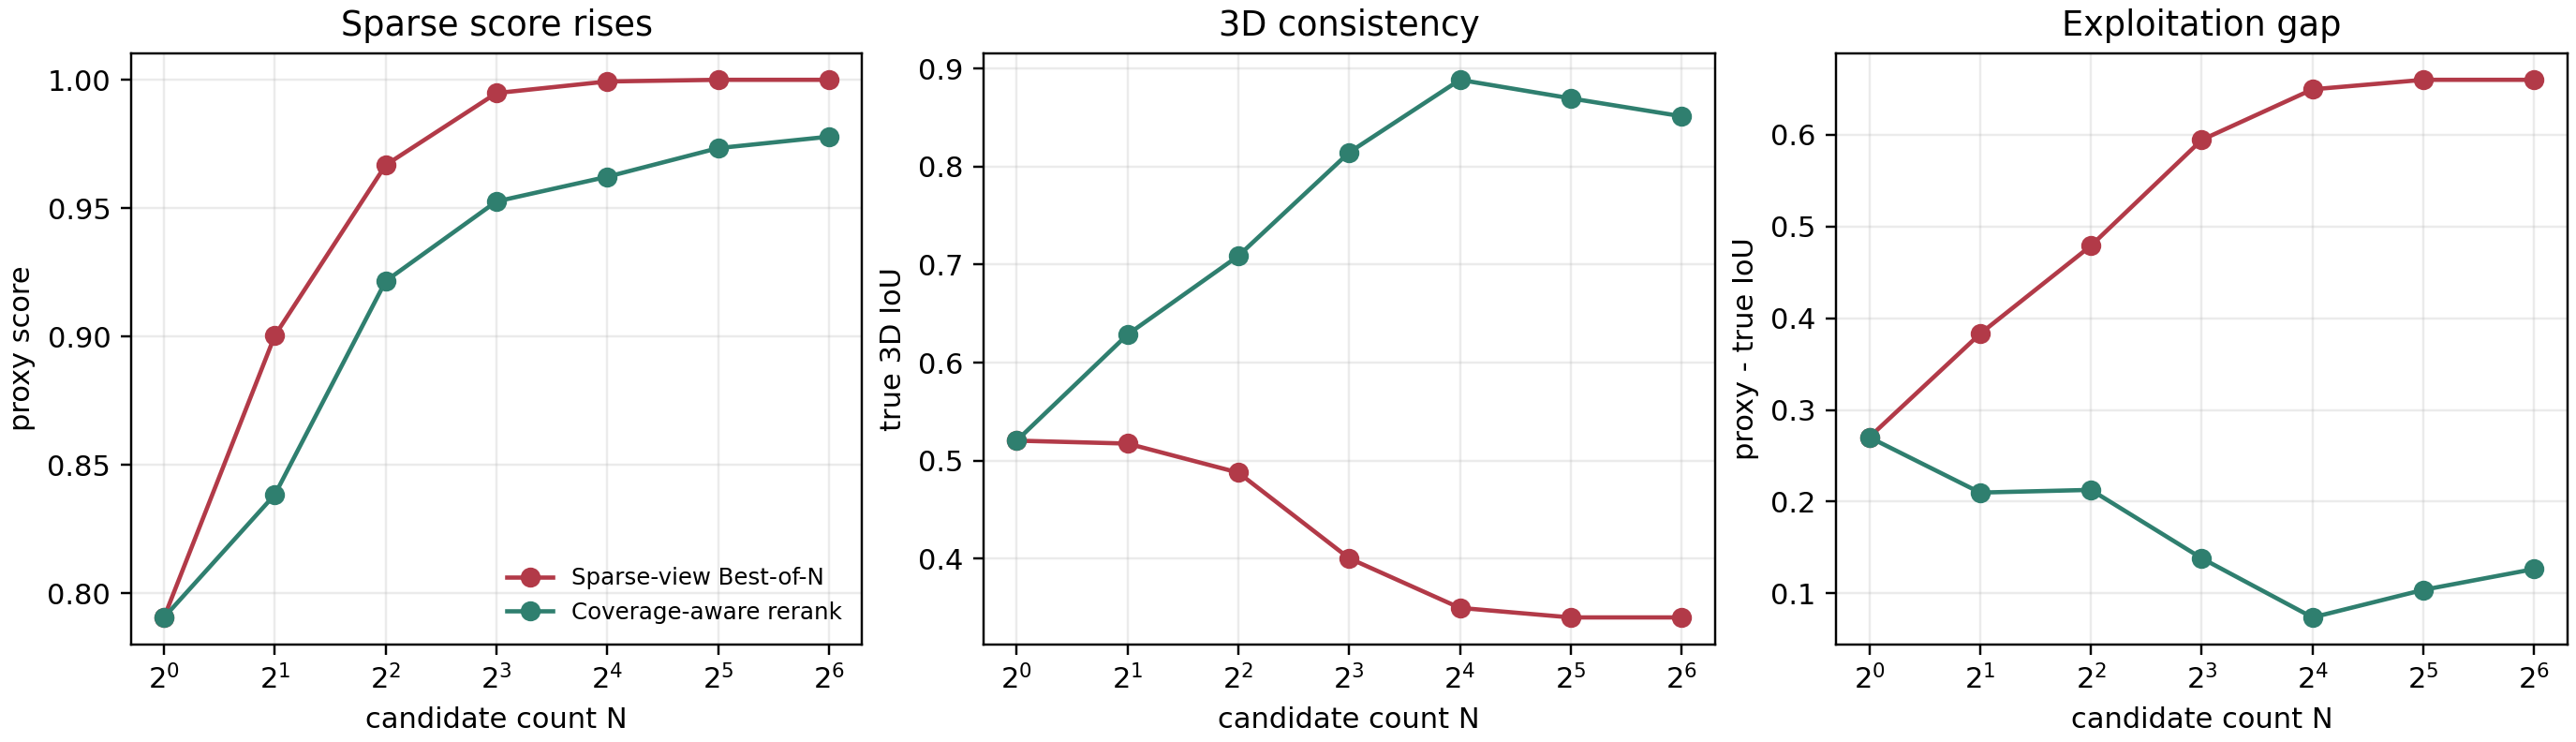
\includegraphics[width=\linewidth]{../figures/bon_tradeoff.png}
  \caption{Naive Best-of-N improves the sparse proxy while reducing true 3D
  consistency. The coverage-aware reranker trades a small amount of proxy score
  for much better 3D IoU and lower exploitation gap.}
  \label{fig:tradeoff}
\end{figure}

\begin{table}[t]
\centering
\caption{Full synthetic run with 72 scenes. Values are means over scenes.}
\label{tab:full}
\begin{tabular}{llrrrr}
\toprule
method & $N$ & proxy & true IoU & hidden error & gap \\
\midrule
naive & 1 & 0.791 & 0.520 & 0.442 & 0.270 \\
naive & 8 & 0.995 & 0.400 & 0.841 & 0.594 \\
naive & 16 & 0.999 & 0.350 & 0.915 & 0.650 \\
naive & 64 & 1.000 & 0.340 & 0.929 & 0.660 \\
\midrule
repaired & 1 & 0.791 & 0.520 & 0.442 & 0.270 \\
repaired & 8 & 0.953 & 0.814 & 0.200 & 0.138 \\
repaired & 16 & 0.962 & 0.888 & 0.121 & 0.074 \\
repaired & 64 & 0.978 & 0.851 & 0.183 & 0.127 \\
\bottomrule
\end{tabular}
\end{table}

The headline result is the divergence between proxy and true 3D consistency.
For naive Best-of-N, proxy score reaches 1.000 at $N=32$ and $N=64$, while true
IoU falls to 0.340. Hidden-region error rises to 0.929. The selected candidate
is a view impostor in 100\% of scenes at $N=32$ and $N=64$.

The repair is not perfect, but it targets the mechanism. It reaches 0.888 true
IoU at $N=16$ and keeps the exploitation gap at 0.074. At $N=64$, the repair
still selects some impostors, but true IoU remains 0.851, far above the naive
0.340.

\begin{figure}[t]
  \centering
  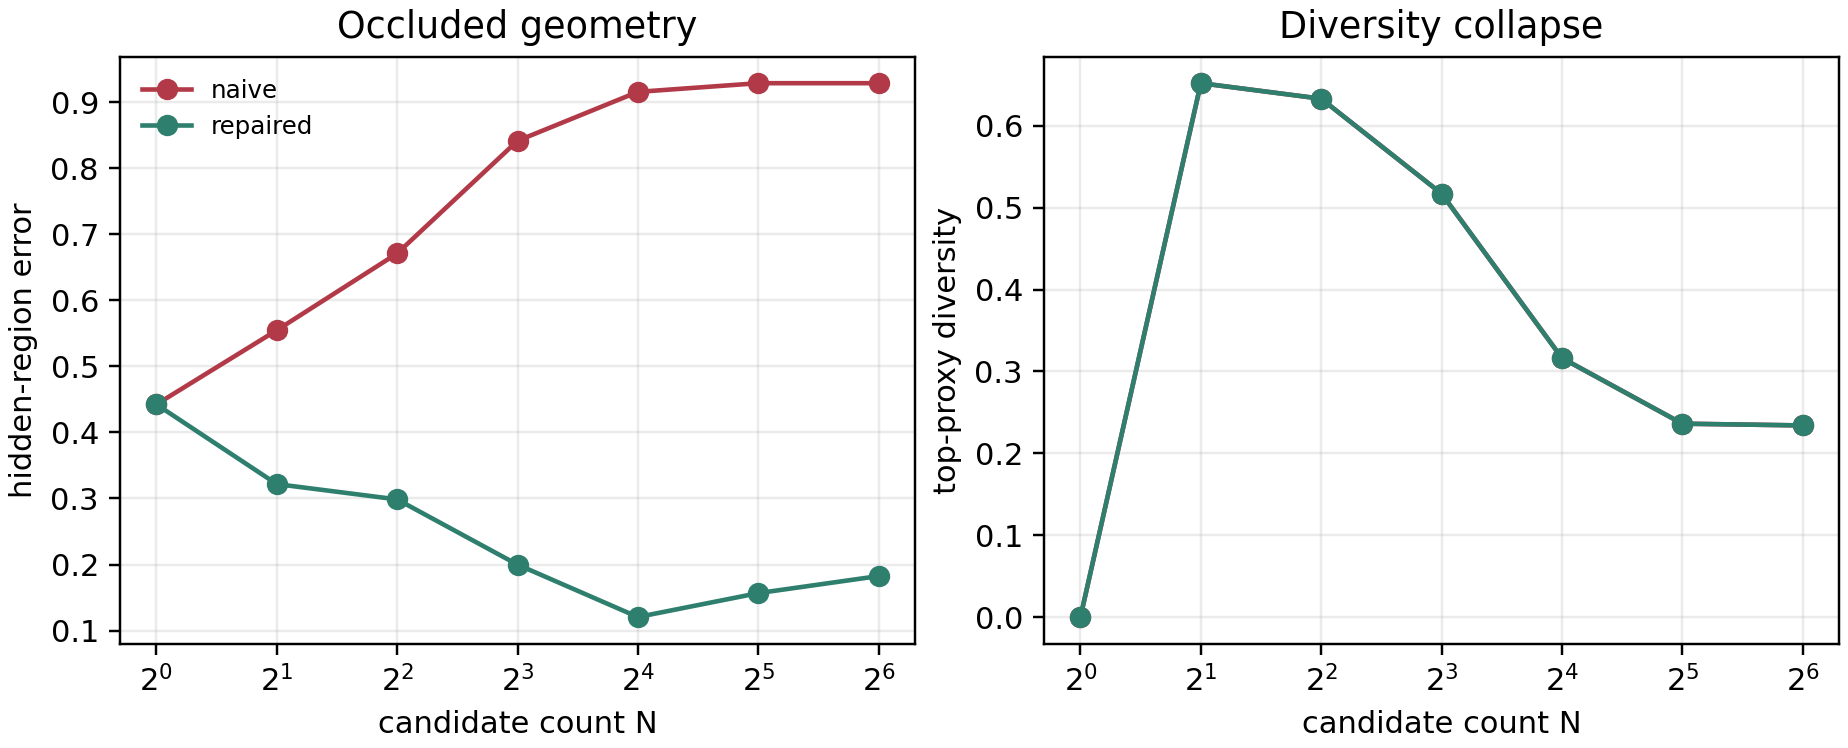
\includegraphics[width=0.82\linewidth]{../figures/hidden_diversity.png}
  \caption{Naive selection increases hidden-region error and collapses
  top-proxy diversity as $N$ grows.}
  \label{fig:hidden}
\end{figure}

\begin{figure}[t]
  \centering
  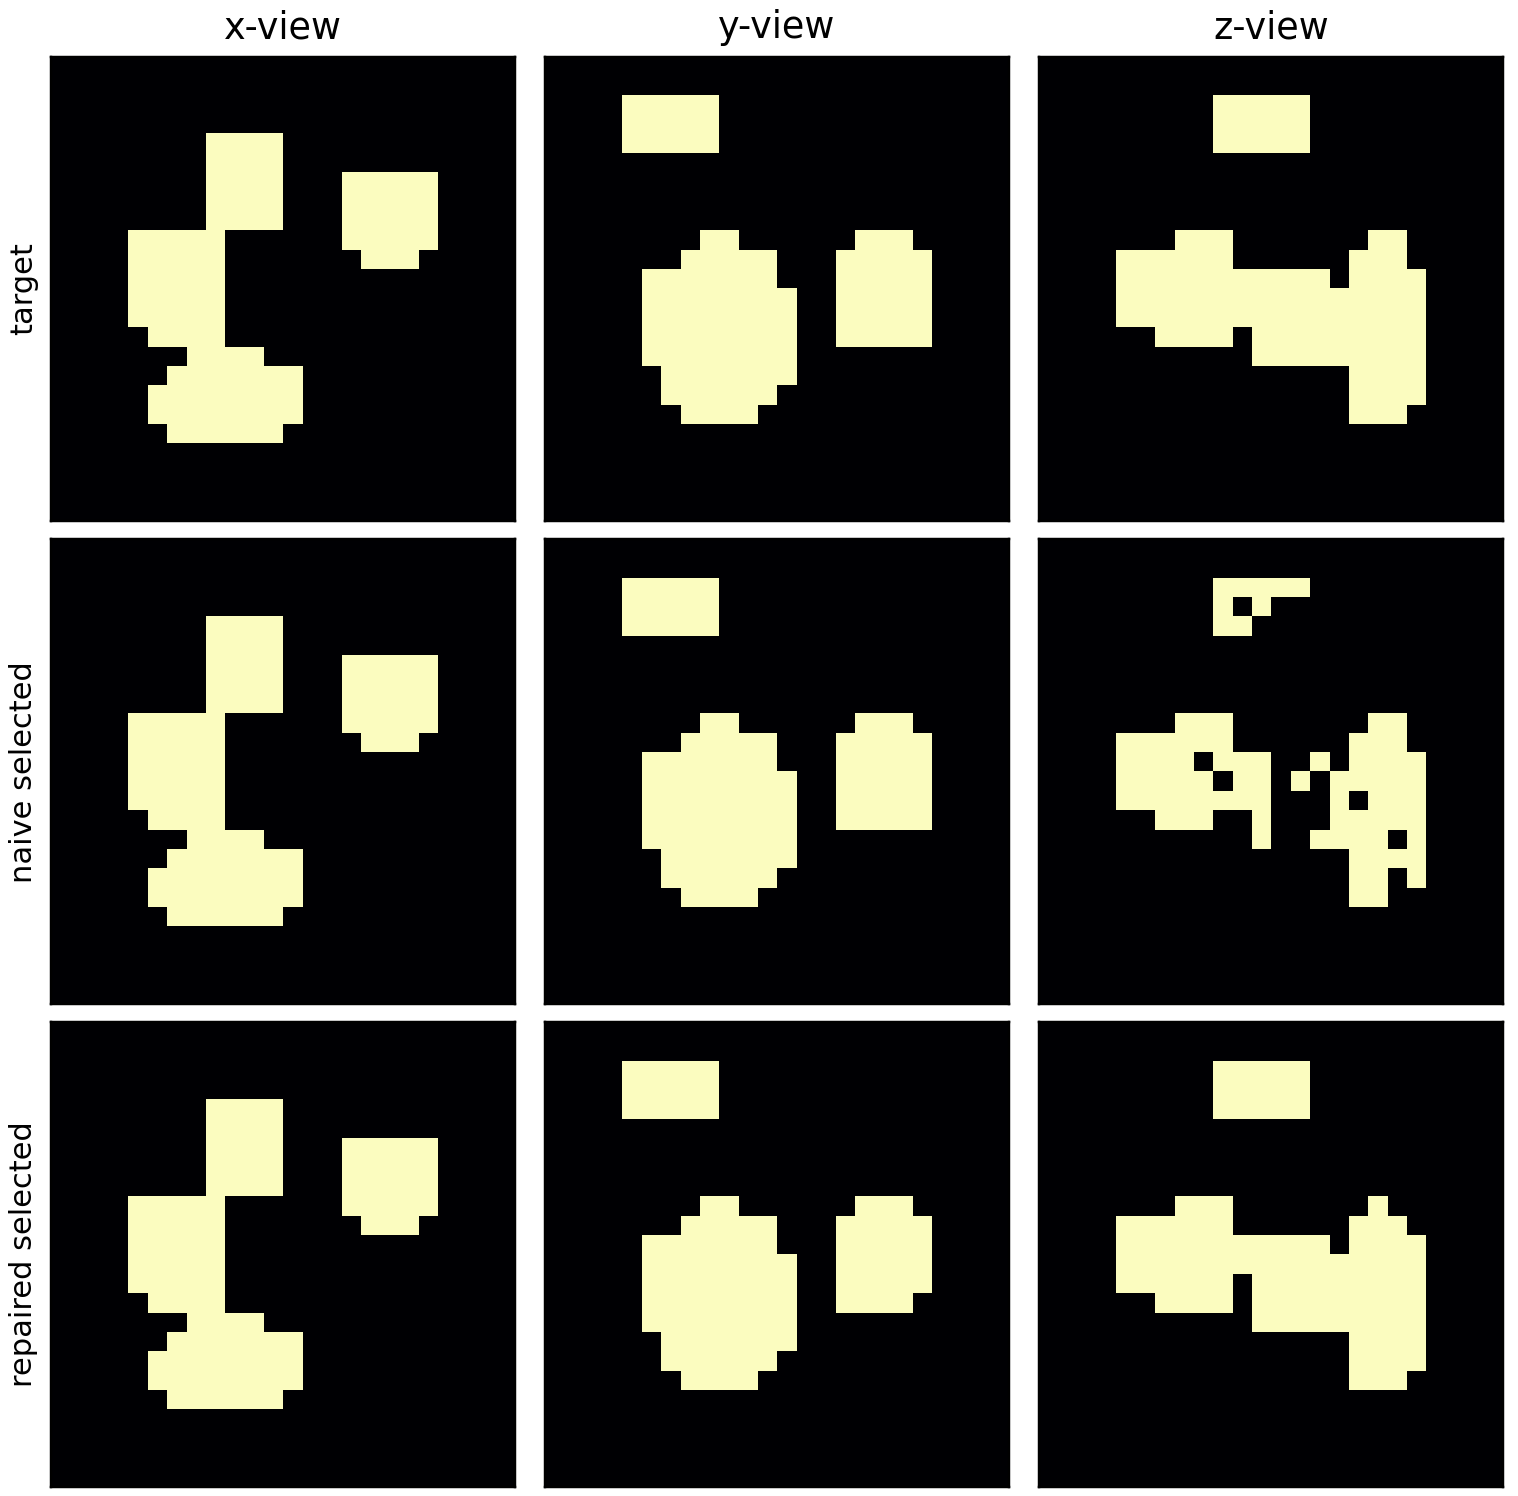
\includegraphics[width=0.72\linewidth]{../figures/example_projections.png}
  \caption{Example projections. The naive selected candidate matches sparse
  scored views but differs in unscored geometry; the repaired candidate preserves
  more global occupancy.}
  \label{fig:example}
\end{figure}

\section{Limitations}

This is a synthetic mechanism study. The candidate sampler is simulated, the
proxy is a simplified silhouette/depth score, and the repair is hand-specified.
The benchmark does not establish failure rates for real NeRF, Gaussian
splatting, point-cloud, or autonomous-driving occupancy systems. The next
submission-quality step is to attach the diagnostic to a real neural-scene
generator and evaluate with held-out 3D reconstructions or multi-view captures.

\section{Reproducibility}

The repository contains deterministic seeds, tests, smoke and full presets, CSV
tables, and generated figures. The main commands are:
\begin{verbatim}
python -m pytest
python experiments/run_synthetic.py --preset smoke --output results/smoke
python experiments/run_synthetic.py --preset full --output results/full
python scripts/build_paper.py
\end{verbatim}

\section{ICLR Checklist}

\textbf{Anonymous submission.} The paper and repository use anonymous author
metadata.

\textbf{Claims.} The claims are limited to the synthetic benchmark and
construction-level mechanism.

\textbf{Code and data.} All benchmark code is included. Data are generated
procedurally.

\textbf{Compute.} Experiments run on CPU. The full preset uses 72 scenes and
finishes in minutes on a standard laptop.

\textbf{Limitations.} The main limitation is lack of real neural-scene
experiments.

\begin{thebibliography}{20}

\bibitem{mildenhall2020nerf}
Mildenhall, B., Srinivasan, P., Tancik, M., Barron, J., Ramamoorthi, R., and Ng, R.
NeRF: Representing scenes as neural radiance fields for view synthesis. ECCV, 2020.

\bibitem{sitzmann2019srn}
Sitzmann, V., Zollhoefer, M., and Wetzstein, G.
Scene representation networks: Continuous 3D-structure-aware neural scene representations. NeurIPS, 2019.

\bibitem{yu2021pixelnerf}
Yu, A., Ye, V., Tancik, M., and Kanazawa, A.
pixelNeRF: Neural radiance fields from one or few images. CVPR, 2021.

\bibitem{wang2021ibrnet}
Wang, Q., Wang, Z., Genova, K., Srinivasan, P., Zhou, H., Barron, J., Martin-Brualla, R., Snavely, N., and Funkhouser, T.
IBRNet: Learning multi-view image-based rendering. CVPR, 2021.

\bibitem{niemeyer2022regnerf}
Niemeyer, M., Barron, J., Mildenhall, B., Sajjadi, M., Geiger, A., and Radwan, N.
RegNeRF: Regularizing neural radiance fields for view synthesis from sparse inputs. CVPR, 2022.

\bibitem{wang2023sparsenerf}
Wang, G., Chen, Z., Loy, C., and Liu, Z.
SparseNeRF: Distilling depth ranking for few-shot novel view synthesis. ICCV, 2023.

\bibitem{kerbl2023gaussian}
Kerbl, B., Kopanas, G., Leimkuehler, T., and Drettakis, G.
3D Gaussian Splatting for real-time radiance field rendering. SIGGRAPH, 2023.

\bibitem{guedon2024sugar}
Guedon, A. and Lepetit, V.
SuGaR: Surface-aligned Gaussian Splatting for efficient 3D mesh reconstruction. CVPR, 2024.

\bibitem{huang2024twodgs}
Huang, B., Yu, Z., Chen, A., Geiger, A., and Gao, S.
2D Gaussian Splatting for geometrically accurate radiance fields. SIGGRAPH, 2024.

\bibitem{mescheder2019occupancy}
Mescheder, L., Oechsle, M., Niemeyer, M., Nowozin, S., and Geiger, A.
Occupancy Networks: Learning 3D reconstruction in function space. CVPR, 2019.

\bibitem{peng2020convocc}
Peng, S., Niemeyer, M., Mescheder, L., Pollefeys, M., and Geiger, A.
Convolutional Occupancy Networks. ECCV, 2020.

\bibitem{cao2022monoscene}
Cao, A. and de Charette, R.
MonoScene: Monocular 3D semantic scene completion. CVPR, 2022.

\bibitem{li2023voxformer}
Li, Y., Yu, Z., Choy, C., Xiao, C., Alvarez, J., Fidler, S., Feng, C., and Anandkumar, A.
VoxFormer: Sparse voxel transformer for camera-based 3D semantic scene completion. CVPR, 2023.

\bibitem{zheng2024occworld}
Zheng, W. et al.
OccWorld: Learning a 3D occupancy world model for autonomous driving. arXiv, 2024.

\bibitem{guzman2012mcl}
Guzman-Rivera, A., Batra, D., and Kohli, P.
Multiple choice learning: Learning to produce multiple structured outputs. NeurIPS, 2012.

\bibitem{bhattacharyya2018best}
Bhattacharyya, A., Fritz, M., and Schiele, B.
Best-of-many samples objective for generative models. CVPR, 2018.

\bibitem{cobbe2021verifiers}
Cobbe, K., Kosaraju, V., Bavarian, M., Chen, M., Jun, H., Kaiser, L., Plappert, M., Tworek, J., Hilton, J., Nakano, R., Hesse, C., and Schulman, J.
Training verifiers to solve math word problems. arXiv, 2021.

\bibitem{lightman2023verify}
Lightman, H. et al.
Let's verify step by step. ICLR, 2023.

\bibitem{laurentini1994visual}
Laurentini, A.
The visual hull concept for silhouette-based image understanding. IEEE TPAMI, 1994.

\bibitem{kutulakos2000space}
Kutulakos, K. and Seitz, S.
A theory of shape by space carving. IJCV, 2000.

\end{thebibliography}

\end{document}
